\title{Reactive Power Compensation Optimization of New Energy Systems Based on Improved Grey Wolf Optimizer}

\author{
\IEEEauthorblockN{Yongwei Zhou}
\IEEEauthorblockA{\textit{Logistics Engineering College} \\
\textit{Shanghai Maritime University} \\
Shanghai 201306, China \\
18216039753@163.com}
\and
\IEEEauthorblockN{Dan Zhang}
\IEEEauthorblockA{\textit{Institute of Logistics Science and Engineering} \\
\textit{Shanghai Maritime University} \\
Shanghai 201306, China \\
zhangdan@shmtu.edu.cn}
\and
\IEEEauthorblockN{Yilian Zhang}
\IEEEauthorblockA{\textit{Institute of Logistics Science and Engineering} \\
\textit{Shanghai Maritime University} \\
Shanghai 201306, China \\
zhanggyl@shmtu.edu.cn}
}

\maketitle

\begin{abstract}
With large-scale wind power integrated into distribution networks, load demand and renewable energy generation exhibit strong time-series fluctuation characteristics. Conventional single-period reactive power compensation strategies frequently lead to issues such as reverse reactive power flow and voltage violation. Existing metaheuristic algorithms suffer from slow convergence, prematurity into local optimum, and difficulty in obtaining stable engineering-feasible solutions when applied to multi-period and high-dimensional reactive power optimization. To address these challenges, this paper presents an improved grey wolf optimizer that combines an adaptive nonlinear convergence factor and a $\delta$-wolf guided fusion mutation mechanism. A multi-period sequential reactive power optimization model is firstly established, which aims to minimize total active power loss, reduce node voltage deviation, and lower the operation cost of reactive power compensation equipment throughout the study period. The model incorporates power flow equality constraints, equipment operation inequality constraints, and practical engineering constraints including capacitor switching operations and OLTC tap change limits. The adopted nonlinear convergence factor dynamically balances global exploration and local exploitation capabilities of the algorithm, while the $\delta$-wolf guided mutation strategy enhances population diversity and suppresses premature convergence. Simulation results verify that the proposed approach effectively reduces active and reactive power losses, smooths operation curves, stabilizes system voltage within a reasonable range, and significantly mitigates voltage fluctuation throughout the entire period. This method provides an effective and practical engineering solution for reactive power optimization and power quality control in distribution networks with high penetration of wind power.
\end{abstract}

\begin{IEEEkeywords}
Grey Wolf Optimizer, Time-Sequential Reactive Power Optimization, Power Quality.
\end{IEEEkeywords}

\section{Introduction}

In distribution networks integrated with wind power generation, the load exhibits significant time-varying fluctuation characteristics throughout the day. Moreover, the temporal mismatch between the daily load profile and wind power output leads to frequent reactive power reverse flow and voltage rise during light-load periods when adopting the conventional single-time snapshot capacitor bank switching strategy. The essence of these issues lies in that the reactive power-voltage control in distribution networks has evolved from static design problems into multi-period, multi-objective, and strongly nonlinear dynamic decision-making problems. Therefore, there is an urgent need for an optimization algorithm that can coordinately regulate reactive power compensation equipment and mitigate all-day voltage deviation.

Metaheuristic algorithms have been widely deployed in power system optimization in recent years, owing to their independence of gradient information and inherent adaptability to mixed-integer programming. Since its proposal in 2014, the Grey Wolf Optimizer (GWO) has been applied in various aspects of energy systems due to its advantages of simple structure and few hyperparameters. Nasir et al.~\cite{b1} summarized more than 200 engineering cases of GWO in optimal power flow (OPF), reactive power dispatch, and equipment sizing in their review.

In terms of algorithm improvement, Meng et al.~\cite{b2} embedded crisscross search into the position update mechanism of GWO, which improved the solution accuracy of the non-convex fuel cost function by about 12\% in the OPF calculation of the IEEE 30-bus system. Abbassi et al.~\cite{b3} proposed a COGWO algorithm by integrating the Levy flight strategy of the cuckoo search into GWO, which reduced the number of iterations by nearly one third in the IEEE 118-bus system with wind power integration. Bouchikhi et al.~\cite{b4} introduced adaptive weights and dynamic encircling factors into GWO, achieving a 69\% reduction in active power loss for the optimal placement and sizing of distributed generation units. Alyu et al.~\cite{b5} integrated the velocity update rule of Particle Swarm Optimization (PSO) into the GWO framework, which improved the voltage deviation index by 18.6\% in the IEEE 33-bus distribution network with multiple photovoltaic (PV) integration.

In the field of device-level control, GWO also shows outstanding advantages in parameter tuning. Nasser et al.~\cite{b6} optimized the Sinusoidal Pulse Width Modulation (SPWM) switching angles of a cascaded multilevel inverter using GWO, which reduced the total harmonic distortion (THD) of the output line voltage from 4.7\% to 2.1\%. Chankaya et al.~\cite{b7} introduced chaotic mapping into GWO for the parameter tuning of the dual-loop Proportional-Integral (PI) controller in a PV-energy storage bidirectional DC-DC converter, which suppressed the DC bus voltage overshoot by 34\%. Gupta et al.~\cite{b8} adopted the standard GWO to tune the Proportional-Integral-Derivative (PID) control parameters of a grid-connected PV inverter, shortening the voltage recovery time to 0.18~s under step changes of irradiance. Wang et al.~\cite{b9} further embedded an improved GWO into the finite control set model predictive control of an LCL-type grid-connected inverter, which controlled the grid-connected current THD within 2.3\% while reducing the switching frequency by 15\%.

In the subdivision field of power quality governance, GWO and its variants have gradually replaced the traditional trial-and-error method for controller parameter optimization and equipment placement and sizing. Ravi and Kumar~\cite{b10} adopted an improved GWO to optimize the regularization coefficient and kernel parameters of a kernel extreme learning machine, achieving a classification accuracy of 97.4\% for 8 types of power quality disturbances including voltage sag, harmonics, and oscillatory transients. Srilakshmi et al.~\cite{b11} proposed a Jaya-GWO hybrid algorithm to optimize the fractional-order PID controller of a three-level hybrid active power filter, which reduced the neutral line current imbalance by 41\% under the electric vehicle charging load scenario. Amini et al.~\cite{b12} optimized the proportional-resonant controller of a shunt active power filter using a genetic algorithm from a comparative perspective, which verified the universality of metaheuristic methods in harmonic suppression.

For the configuration of reactive power compensation devices, Rao et al.~\cite{b13} applied multi-objective GWO to the optimal placement and sizing of a Thyristor-Controlled Series Capacitor (TCSC), and obtained the Pareto front of power loss and investment cost in the IEEE 30-bus system. Rajakumar et al.~\cite{b14} adopted the osprey optimization algorithm for the coordinated planning of PV units and capacitor banks, which reduced the active power loss by 75.1\%. Mahmoud et al.~\cite{b15} combined GWO with Levy flight for the first time to complete the 24-hour sequential voltage control optimization in the IEEE 123-bus unbalanced distribution network with high PV penetration, which reduced the daily average voltage unbalance factor (VUF) from 2.3\% to 1.6\%. This work marks that the application of GWO in the power quality field has extended from single-snapshot static optimization to multi-period dynamic decision-making.

However, the above-mentioned works still have two critical shortcomings in solving the all-day reactive power compensation problem. Firstly, the convergence factor of most existing GWO variants generally adopts a linear decreasing law, which leads to excessively fast shrinkage of the global exploration radius in the early search stage and insufficient local exploitation accuracy in the later stage. Secondly, the individual position update in the standard GWO is only guided by the weighted sum of the three leading wolves, namely $\alpha$, $\beta$, and $\delta$ wolves; there is no mechanism to reconstruct the guiding direction by fusing the historical optimal information of the three elite individuals. These two limitations make it difficult for existing GWO algorithms to stably converge to engineering-feasible solutions in practical 24-hour reactive power optimization with multiple discrete control devices (a five-step capacitor bank and a nine-tap OLTC) and strong cross-time coupling constraints.

To address the above shortcomings, this paper proposes an improved grey wolf optimizer (IGWO) integrating a polynomial-decay convergence factor and a $\delta$-wolf guided fusion mutation strategy, applied to the all-day reactive power compensation optimization of wind-integrated distribution networks. A multi-period reactive power compensation model is established with the optimization objectives of minimizing the daily total active power loss, split voltage deviation (rise and drop), and cross-time reactive power variation, while enforcing practical constraints including reactive power circle limits, discrete capacitor switching operations, and OLTC tap change limits. The proposed IGWO is adopted to coordinately solve the 24-hour reactive power dispatch curves. This work aims to provide an engineering-feasible optimization solution for dynamic power quality governance of distribution networks with high penetration of renewable energy.

\section{Mathematical Model}

\subsection{Power Flow Model for Radial Distribution Networks}

The IEEE 33-bus test system is a radial distribution network with a single slack bus (node 0) and 32 PQ nodes. Given the radial topology, the backward-forward sweep (BFS) method is adopted for power flow calculation. The node injection complex power $\boldsymbol{S}$ relates to the node voltage $\boldsymbol{V}$ and admittance matrix $\boldsymbol{Y}$ through
\begin{equation}
\boldsymbol{S} = \boldsymbol{V} \cdot \left(\boldsymbol{Y}\boldsymbol{V}\right)^*
\end{equation}
where $\boldsymbol{S}_i = P_i + jQ_i$ is the net complex power injected at node $i$.

The BFS method iterates between two sweeps. In the backward sweep, the branch current flowing from node $i$ toward node $j$ (away from the substation) is computed by summing the load current at node $j$ and all downstream branch currents:
\begin{equation}
I_{ij}^{(k)} = \frac{P_j - jQ_j}{V_j^{(k)*}} + \sum_{c \in \text{children}(j)} I_{jc}^{(k)}
\label{eq:bfs_backward}
\end{equation}
In the forward sweep, node voltages are updated from the substation outward:
\begin{equation}
V_j^{(k+1)} = V_i^{(k+1)} - Z_{ij} \cdot I_{ij}^{(k)}
\label{eq:bfs_forward}
\end{equation}
where $Z_{ij} = R_{ij} + jX_{ij}$ is the branch impedance. The iteration proceeds until the maximum voltage magnitude change between successive sweeps falls below $10^{-8}$~pu.

The active power loss on each branch is computed from the converged branch current:
\begin{equation}
\Delta P_{ij} = \left|I_{ij}\right|^2 R_{ij}
\label{eq:line_loss}
\end{equation}

\subsection{Multi-Objective Optimization Formulation}

The all-day reactive power dispatch problem minimizes a composite objective over $H=24$ hourly periods. The decision vector comprises six device categories---three wind turbines (WT1--WT3), one SVG, one capacitor bank, and one OLTC---yielding $6 \times 24 = 144$ continuous decision variables.

\subsubsection{Objective Components}

\textit{Active power loss} ($f_1$): Total daily active power loss summed over all lines:
\begin{equation}
f_1 = \sum_{h=1}^{24} \sum_{(i,j) \in \mathcal{L}} G_{ij}\Bigl(V_i^2(h) + V_j^2(h) - 2V_i(h)V_j(h)\cos\theta_{ij}(h)\Bigr)
\label{eq:f1_active_loss}
\end{equation}
where $\mathcal{L}$ is the set of branches, $G_{ij}$ the branch conductance, and $\theta_{ij}(h)=\theta_i(h)-\theta_j(h)$.

\textit{Voltage deviation} ($f_2$): The voltage deviation at each node is split into rise and drop components with respect to the reference $V_{\text{ref}}=1.0$~pu, weighted separately to penalize voltage drops more heavily:
\begin{equation}
\begin{aligned}
f_{2,\text{rise}} &= \sum_{h=1}^{24} \sum_{i=1}^{n} \max\!\bigl(V_i(h) - V_{\text{ref}},\; 0\bigr)^2 \\
f_{2,\text{drop}} &= \sum_{h=1}^{24} \sum_{i=1}^{n} \max\!\bigl(V_{\text{ref}} - V_i(h),\; 0\bigr)^2
\end{aligned}
\label{eq:f2_voltage}
\end{equation}

\textit{Cross-time reactive power variation} ($\Delta Q$): To avoid excessive actuator wear and to encourage temporally smooth dispatch, a time-coupling penalty weighted by the load level $w(h)$ is introduced:
\begin{equation}
\Delta Q = \sum_{h=1}^{23} w(h) \sum_{d=1}^{n_Q} \Bigl(Q_d(h+1) - Q_d(h)\Bigr)^2
\label{eq:delta_q}
\end{equation}
where $n_Q$ counts the continuously adjustable reactive power devices (WT1--WT3 and SVG), and $w(h)$ is the normalized load ratio at hour $h$.

\subsubsection{Composite Objective}

The comprehensive fitness function combines the above components with penalty terms for constraint violations:
\begin{equation}
\begin{aligned}
\min F = &\;\; w_1 f_1 + w_{2,\text{rise}} f_{2,\text{rise}} + w_{2,\text{drop}} f_{2,\text{drop}} + w_3 \Delta Q \\
        &+ \lambda \cdot \Phi_V + \mu \cdot \Phi_Q + \Phi_{\text{cap}} + \Phi_{\text{OLTC}}
\label{eq:comprehensive_objective}
\end{aligned}
\end{equation}
where the weight coefficients are set as $w_1=0.30$, $w_{2,\text{rise}}=0.15$, $w_{2,\text{drop}}=0.30$, and $w_3=0.03$.

\subsection{Constraints}

\textit{Voltage limits} (GB/T standard): All node voltages must remain within $[0.90,\,1.10]$~pu. Violations incur a quadratic penalty:
\begin{equation}
\Phi_V = \sum_{h=1}^{24} \sum_{i=1}^{n} \Bigl[\max\!\bigl(V_{\min} - V_i(h),\,0\bigr)^2 + \max\!\bigl(V_i(h) - V_{\max},\,0\bigr)^2\Bigr]
\label{eq:voltage_penalty}
\end{equation}
with $\lambda = 200$.

\textit{Reactive power circle constraint}: For each wind turbine and the SVG, the reactive power output is bounded by the apparent power rating and the active power output at each hour:
\begin{equation}
Q_{d}^2(h) \leq S_{d}^2 - P_{d}^2(h), \quad d \in \{\text{WT1, WT2, WT3, SVG}\}
\label{eq:circle_constraint}
\end{equation}
Violations are penalized with $\mu = 100$:
\begin{equation}
\Phi_Q = \sum_{h=1}^{24} \sum_{d} \max\!\bigl(|Q_d(h)| - \sqrt{S_d^2 - P_d^2(h)},\; 0\bigr)^2
\label{eq:circle_penalty}
\end{equation}

\textit{Device capacity bounds}:
\begin{equation}
\begin{cases}
Q_{\text{WT},k}^{\min} \leq Q_{\text{WT},k} \leq Q_{\text{WT},k}^{\max}, & k=1,2,3 \\[2pt]
Q_{\text{SVG}}^{\min} \leq Q_{\text{SVG}} \leq Q_{\text{SVG}}^{\max} \\[2pt]
0 \leq Q_{\text{cap}} \leq Q_{\text{cap}}^{\max}
\end{cases}
\label{eq:device_bounds}
\end{equation}

\textit{Discrete capacitor switching}: The capacitor bank is divided into 5 equal steps of 0.03~pu each (total 0.15~pu). The continuous decision variable is rounded to the nearest step during evaluation. The number of daily switching operations is limited to $N_{\text{cap}}^{\max}=5$:
\begin{equation}
\Phi_{\text{cap}} = \lambda_{\text{cap}} \cdot \max\!\Bigl(0,\; \sum_{h=1}^{23} \mathbb{1}\bigl[|Q_{\text{cap}}(h+1)-Q_{\text{cap}}(h)|>\epsilon\bigr] - N_{\text{cap}}^{\max}\Bigr)
\label{eq:cap_penalty}
\end{equation}

\textit{OLTC tap constraints}: The on-load tap changer at the substation has 9 integer tap positions ($-4$ to $+4$), each providing a $\pm 2.5\%$ voltage adjustment. The continuous decision variable is rounded to the nearest integer. Daily tap changes are capped at $N_{\text{OLTC}}^{\max}=6$:
\begin{equation}
V_{\text{slack}}(h) = 1.0 + \text{tap}(h) \times 0.025,\quad \text{tap}(h) \in \{-4,-3,\ldots,4\}
\label{eq:oltc_model}
\end{equation}
Excessive tap operations are penalized analogously to \eqref{eq:cap_penalty} with $\lambda_{\text{OLTC}}=6$.

\section{Improved Grey Wolf Optimizer}

The proposed Improved Grey Wolf Optimizer (IGWO) incorporates three enhancements over the standard GWO: (i)~nonlinear convergence factor for adaptive exploration--exploitation balance, (ii)~$\delta$-wolf fusion mutation for diversity preservation, and (iii)~unequal position-update weights for guided convergence.

\subsection{Logistic Chaotic Initialization}

To improve initial population diversity in the 144-dimensional search space, a logistic chaotic map replaces uniform random initialization:
\begin{equation}
r_{d}^{(i+1)} = 4.0 \cdot r_{d}^{(i)} \cdot \bigl(1 - r_{d}^{(i)}\bigr)
\label{eq:logistic_init}
\end{equation}
\begin{equation}
X_{i,d}(0) = X_d^{\min} + r_{d}^{(i)} \cdot \bigl(X_d^{\max} - X_d^{\min}\bigr),\quad d=1,\ldots,144
\label{eq:init_position}
\end{equation}
where $r_d^{(0)}\sim U(0,1)$ is independently drawn for each dimension $d$, and the logistic map is iterated once per grey wolf $i$.

\subsection{Nonlinear Convergence Factor}

The standard GWO uses a linearly decreasing convergence factor $a = 2(1 - m/M)$, which provides equal emphasis on exploration and exploitation throughout the search. IGWO replaces it with a polynomial-decay factor:
\begin{equation}
a(m) = a_0 - \lambda \cdot \left(\frac{m}{M}\right)^k
\label{eq:nonlinear_a}
\end{equation}
where $a_0=2.0$, $\lambda=1.8$, $k=1.0$, $m$ is the current iteration, and $M$ is the maximum iteration count. With $k=1$, $a$ decreases from 2.0 to 0.2, providing a linear schedule that can be tuned to nonlinear ($k>1$) for stronger late-stage exploitation when needed.

\subsection{$\delta$-Wolf Fusion Mutation}

In standard GWO, the $\delta$ wolf is simply the third-best individual. IGWO generates a \textit{fused} $\delta$ wolf through weighted averaging of the top three wolves, giving higher influence to the $\alpha$ and $\beta$ leaders:
\begin{equation}
\vec{X}_{\delta}^{\text{new}} = \frac{w_\alpha \vec{X}_\alpha + w_\beta \vec{X}_\beta + w_\delta \vec{X}_\delta}{w_\alpha + w_\beta + w_\delta}
\label{eq:delta_fusion}
\end{equation}
with $w_\alpha = 0.50$, $w_\beta = 0.33$, $w_\delta = 0.17$. This fused leader replaces the original $\delta$ wolf in the position update, pulling the population toward a refined search direction that blends information from all three elite individuals.

\subsection{Position Update with Unequal Weights}

Each $\omega$ wolf updates its position by computing three candidate positions relative to $\alpha$, $\beta$, and the fused $\delta$ wolf:
\begin{equation}
\begin{aligned}
\vec{D}_\alpha &= \bigl|\vec{C}_1 \odot \vec{X}_\alpha - \vec{X}\bigr|, \quad
\vec{X}_1 = \vec{X}_\alpha - \vec{A}_1 \odot \vec{D}_\alpha \\
\vec{D}_\beta  &= \bigl|\vec{C}_2 \odot \vec{X}_\beta  - \vec{X}\bigr|, \quad
\vec{X}_2 = \vec{X}_\beta  - \vec{A}_2 \odot \vec{D}_\beta \\
\vec{D}_\delta &= \bigl|\vec{C}_3 \odot \vec{X}_\delta^{\text{new}} - \vec{X}\bigr|, \;
\vec{X}_3 = \vec{X}_\delta^{\text{new}} - \vec{A}_3 \odot \vec{D}_\delta
\end{aligned}
\label{eq:candidate_positions}
\end{equation}
where $\odot$ denotes element-wise multiplication. The coefficient vectors follow the standard GWO formulation:
\begin{equation}
\vec{A}_j = 2a \cdot \vec{r}_{j,1} - a,\qquad
\vec{C}_j = 2 \cdot \vec{r}_{j,2},\quad j=1,2,3
\label{eq:coefficient_vectors}
\end{equation}
with $\vec{r}_{j,1}, \vec{r}_{j,2} \sim U(0,1)$.

The final position is obtained through an unequal weighted average that assigns the highest weight to the $\alpha$-guided direction:
\begin{equation}
\vec{X}(m+1) = 0.50\,\vec{X}_1 + 0.30\,\vec{X}_2 + 0.20\,\vec{X}_3
\label{eq:position_update}
\end{equation}
This is in contrast to standard GWO, which uses an equal-weight average $(\vec{X}_1+\vec{X}_2+\vec{X}_3)/3$. After updating, the position is clipped to the feasible box $[X^{\min}, X^{\max}]$. The iterative process repeats until the maximum number of iterations $M$ is reached, after which the $\alpha$ wolf position is decoded into the optimal 24-hour reactive power dispatch schedule.

\section{Simulation Results}

The proposed IGWO algorithm is evaluated on the IEEE 33-bus radial distribution test system (12.66~kV, 10~MVA base) with three wind turbines (1.2/1.2/0.8~MW), a $\pm$2.5~MVar SVG, a 0--1.5~MVar five-step capacitor bank, and a $\pm$10\% OLTC at the substation. The 24-hour dispatch problem involves 144 decision variables (6 devices $\times$ 24 hours). All algorithms employ a population size of 20; Standard GWO runs for 150 iterations and IGWO for 300 iterations.

Table~\ref{tab:results} summarizes the optimization results. The baseline case (all reactive power set to zero) yields an active power loss of 0.1849~pu, a reactive power loss of 0.1368~pu, and a voltage deviation of 0.4390. Standard GWO reduces the active loss by 11.6\% and the voltage deviation by 56.3\%. The proposed IGWO achieves the best performance across all metrics: active power loss drops to 0.1361~pu ($-$26.4\%), reactive power loss to 0.1086~pu ($-$20.6\%), and voltage deviation to 0.1583 ($-$63.9\%). Compared with Standard GWO, IGWO improves the composite fitness by 23.4\%.

\begin{table}[!t]
  \centering
  \caption{Optimization Results on the IEEE 33-Bus System}
  \label{tab:results}
  \begin{tabular}{lcccc}
    \hline
    Method & P$_{\text{loss}}$ (pu) & Q$_{\text{loss}}$ (pu) & V$_{\text{dev}}$ & Fitness \\
    \hline
    Baseline (Q=0)  & 0.1849 & 0.1368 & 0.4390 & -- \\
    Standard GWO    & 0.1635 & 0.1266 & 0.1920 & 0.1006 \\
    \textbf{Improved GWO} & \textbf{0.1361} & \textbf{0.1086} & \textbf{0.1583} & \textbf{0.0770} \\
    \hline
  \end{tabular}
\end{table}

Fig.~\ref{fig:active_loss} presents the hourly active power loss profiles. The baseline curve follows the load profile, peaking at approximately 0.0094~pu during the evening peak period (19:00--20:00). Standard GWO moderately reduces losses but exhibits a higher peak (0.0098~pu) due to suboptimal reactive power allocation in certain hours, indicating that the standard algorithm struggles with the 144-dimensional coupled search space. The proposed IGWO achieves substantial loss reductions during daytime hours (08:00--20:00), with per-hour improvements of 30\%--57\% over the baseline. A modest trade-off is observed in early morning hours (00:00--06:00), where IGWO applies mild reactive compensation for voltage regulation, resulting in marginally higher losses in 5 of 24 periods (maximum $+5.3$\%, excluding one transitional hour at the wind-load crossover point). This trade-off reflects the multi-objective nature of the formulation: under low-load, high-wind conditions, voltage rise suppression takes priority over loss minimization.

Fig.~\ref{fig:voltage_deviation} compares the voltage deviation index $\sum (V_i - V_{\text{ref}})^2$ across the three cases. The baseline curve remains elevated throughout the day, with a peak exceeding 0.039, confirming that unregulated reactive power flow severely degrades voltage quality in high-penetration wind scenarios. Standard GWO partially mitigates the deviation (peak reduced to 0.035) but retains noticeable fluctuations. IGWO drives the maximum deviation down to 0.017, a 57\% reduction from the baseline peak, and maintains the lowest profile across all 24 hours. This superior voltage regulation stems from the coordinated dispatch of the SVG, capacitor bank, and OLTC, enabled by IGWO's enhanced global search capability through the nonlinear convergence factor and $\delta$-wolf fusion mutation.

Fig.~\ref{fig:reactive_loss} shows the reactive power loss comparison. The baseline reactive loss profile exhibits pronounced peaks during the evening load surge, indicating excessive reactive current circulation in the distribution lines. Standard GWO achieves a moderate reduction in total reactive loss but produces a slightly elevated peak (0.0078~pu vs.\ 0.0071~pu baseline), again reflecting inadequate convergence in the coupled 24-hour optimization. IGWO delivers the best overall reduction ($-$20.6\% total) and the most flattened daily profile, confirming its ability to allocate reactive compensation resources efficiently across all time periods.

The convergence behavior, shown in Fig.~\ref{fig:convergence}, reveals that IGWO diverges from Standard GWO around iteration 40 and consistently converges to a lower fitness plateau (0.0770 vs.\ 0.1006). The nonlinear convergence factor $a(m) = a_0 - \lambda (m/M)^k$ provides stronger exploration in early iterations and faster exploitation in later stages, while the $\delta$-wolf fusion mutation maintains population diversity to prevent premature stagnation.

\begin{figure}[!t]
  \centering
  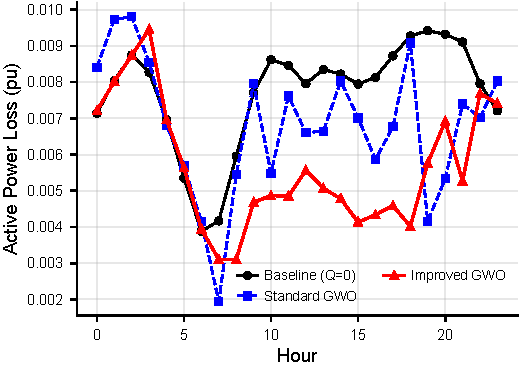
\includegraphics[width=0.85\linewidth]{fig1_active_power_loss.pdf}
  \caption{Active power loss comparison among Baseline (Q=0), Standard GWO, and Improved GWO on the IEEE 33-bus system.}
  \label{fig:active_loss}

  \vspace{8pt}

  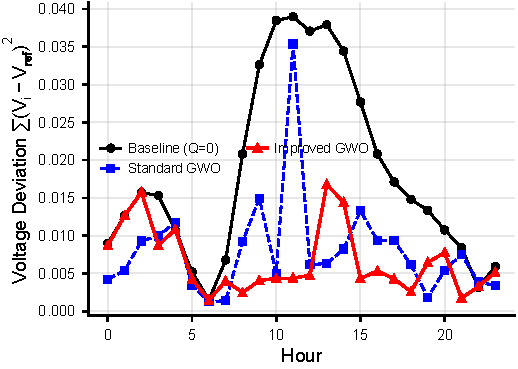
\includegraphics[width=0.85\linewidth]{fig2_voltage_deviation.pdf}
  \caption{Voltage deviation comparison among Baseline (Q=0), Standard GWO, and Improved GWO.}
  \label{fig:voltage_deviation}

  \vspace{8pt}

  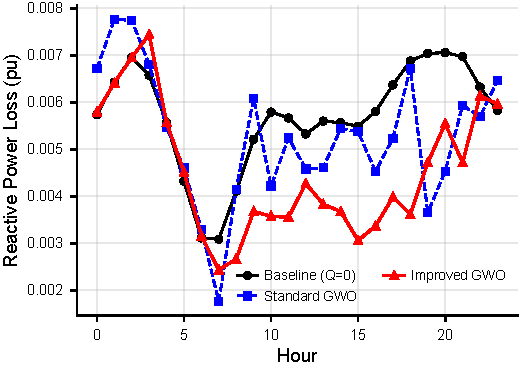
\includegraphics[width=0.85\linewidth]{fig3_reactive_power_loss.pdf}
  \caption{Reactive power loss comparison among Baseline (Q=0), Standard GWO, and Improved GWO.}
  \label{fig:reactive_loss}
\end{figure}

\begin{figure}[!t]
  \centering
  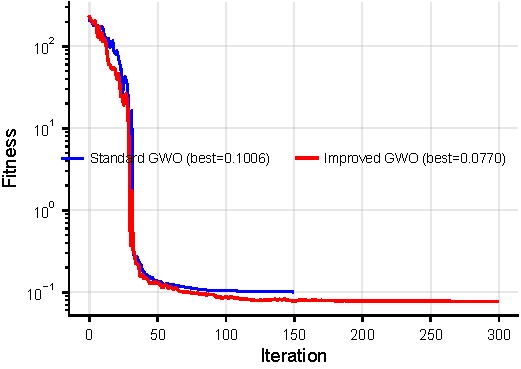
\includegraphics[width=0.85\linewidth]{fig4_convergence.pdf}
  \caption{Convergence curves of Standard GWO and Improved GWO on the IEEE 33-bus system.}
  \label{fig:convergence}
\end{figure}

\section{Conclusion}

This paper has presented an improved grey wolf optimizer for the all-day sequential reactive power dispatch problem in wind-integrated distribution networks. A multi-objective optimization model was established that simultaneously minimizes active power loss, voltage deviation (split into rise and drop components), and cross-time reactive power variation, while enforcing practical engineering constraints including reactive power circle limits, discrete capacitor switching operations, and OLTC tap change limits. The IGWO incorporates three targeted enhancements: a polynomial-decay convergence factor for adaptive exploration--exploitation balancing, a $\delta$-wolf fusion mutation that blends elite individual information to preserve population diversity, and unequal position-update weights that strengthen guidance from the $\alpha$-wolf direction.

Simulation on the IEEE 33-bus system with three wind turbines, one SVG, one five-step capacitor bank, and one nine-tap OLTC demonstrates that IGWO reduces total active power loss by 26.4\%, reactive power loss by 20.6\%, and voltage deviation by 63.9\% relative to the uncompensated baseline, outperforming Standard GWO by 23.4\% in composite fitness. The hourly profiles confirm that IGWO achieves substantial improvements during daytime peak-load hours while accepting a modest trade-off in early-morning low-load periods for superior voltage regulation. These results validate that the proposed algorithm provides an efficient and engineering-feasible solution for dynamic reactive power management in distribution systems with high renewable penetration. Future work will extend the framework to multi-time-scale optimization and source--grid--load--storage coordination in hybrid AC/DC networks.

\begin{thebibliography}{1}

\bibitem{b1} M.~Nasir, A.~Sadollah, S.~Mirjalili, S.~A.~Mansouri, M.~Safaraliev, and A.~R.~Jordehi, ``A Comprehensive Review on Applications of Grey Wolf Optimizer in Energy Systems,'' \textit{Arch. Comput. Methods Eng.}, vol.~32, no.~4, pp.~2279--2319, May~2025, doi: 10.1007/s11831-024-10214-3.

\bibitem{b2} A.~Meng, C.~Zeng, P.~Wang, D.~Chen, T.~Zhou, X.~Zheng, and H.~Yin, ``A high-performance crisscross search based grey wolf optimizer for solving optimal power flow problem,'' \textit{Energy}, vol.~225, Art.~no.~120211, Jun.~2021, doi: 10.1016/j.energy.2021.120211.

\bibitem{b3} R.~Abbassi, P.~Trojovsk\'{y}, Z.~Mansor, E.~Trojovsk\'{a}, M.~Kchaou, T.~Zu\v{s}\v{c}\'{a}k, H.~Jerbi, and P.~Naveen, ``Cuckoo optimization algorithm via Grey Wolf Optimizer for usage in engineering optimization and optimal power flow with renewable energy sources,'' \textit{Sci. Rep.}, vol.~15, no.~1, pp.~1--37, Oct.~2025, doi: 10.1038/s41598-025-21515-3.

\bibitem{b4} N.~Bouchikhi, F.~Boussadia, R.~Bouddou, A.~O.~Salau, S.~Mekhilef, C.~Gouder, S.~Adiche, and A.~Belabbes, ``Optimal distributed generation placement and sizing using modified grey wolf optimization and ETAP for power system performance enhancement and protection adaptation,'' \textit{Sci. Rep.}, vol.~15, no.~1, pp.~1--31, Apr.~2025, doi: 10.1038/s41598-025-98012-0.

\bibitem{b5} A.~B.~Alyu, A.~O.~Salau, B.~Khan, and J.~N.~Eneh, ``Hybrid GWO-PSO based optimal placement and sizing of multiple PV-DG units for power loss reduction and voltage profile improvement,'' \textit{Sci. Rep.}, vol.~13, no.~1, pp.~1--17, Apr.~2023, doi: 10.1038/s41598-023-34057-3.

\bibitem{b6} A.~M.~Nasser, A.~Refky, H.~Shatla, and A.~M.~Abdel-hamed, ``A grey wolf optimization-based modified SPWM control scheme for a three-phase half bridge cascaded multilevel inverter,'' \textit{Sci. Rep.}, vol.~14, no.~1, pp.~1--33, Mar.~2024, doi: 10.1038/s41598-024-57262-0.

\bibitem{b7} M.~Chankaya, M.~Aijaz, M.~Panda, I.~Hussain, and B.~Singh, ``Chaotic Grey Wolf Optimized DC-DC Bi-Directional Converter for a Single-Phase Grid-Tied PV-BES System,'' \textit{IEEE Trans. Ind. Appl.}, vol.~62, no.~1, pp.~1516--1527, Jan.~2026, doi: 10.1109/TIA.2025.3603513.

\bibitem{b8} M.~Gupta, P.~M.~Tiwari, R.~K.~Viral, A.~Shrivastava, B.~Abu~Zneid, and I.~Hunko, ``Grid-connected PV inverter system control optimization using Grey Wolf optimized PID controller,'' \textit{Sci. Rep.}, vol.~15, no.~1, pp.~1--31, Aug.~2025, doi: 10.1038/s41598-025-10617-7.

\bibitem{b9} F.~Wang, F.~Cai, D.~Huang, Y.~Wei, D.~Ke, and Z.~Zhang, ``Multiobjective Model Predictive Control of LCL Grid-Connected Inverter Based on an Improved Gray Wolf Algorithm,'' \textit{IEEE Trans. Power Electron.}, vol.~40, no.~9, pp.~13977--13990, Sep.~2025, doi: 10.1109/TPEL.2025.3572213.

\bibitem{b10} T.~Ravi and K.~S.~Kumar, ``Detection and Classification of Power Quality Disturbances Using Stock Well Transform and Improved Grey Wolf Optimization-Based Kernel Extreme Learning Machine,'' \textit{IEEE Access}, vol.~11, pp.~61710--61727, Jun.~2023, doi: 10.1109/ACCESS.2023.3286308.

\bibitem{b11} K.~Srilakshmi, D.~T.~Santosh, A.~Ramadevi, P.~K.~Balachandran, G.~P.~Reddy, A.~Palanivelu, I.~Colak, C.~Dhanamjayulu, R.~K.~Chinthaginjala, and B.~Khan, ``Development of renewable energy fed three-level hybrid active filter for EV charging station load using Jaya grey wolf optimization,'' \textit{Sci. Rep.}, vol.~14, no.~1, pp.~1--23, Feb.~2024, doi: 10.1038/s41598-024-54550-7.

\bibitem{b12} B.~Amini, H.~Rastegar, and M.~Pichan, ``An optimized proportional resonant current controller based genetic algorithm for enhancing shunt active power filter performance,'' \textit{Int. J. Electr. Power Energy Syst.}, vol.~156, Art.~no.~109738, Feb.~2024, doi: 10.1016/j.ijepes.2023.109738.

\bibitem{b13} N.~T.~Rao, K.~K.~Kumar, P.~P.~Kumar, R.~S.~S.~Nuvvula, A.~Mutharasan, C.~Dhanamjayulu, M.~R.~Shaik, and B.~Khan, ``Multiobjective optimal TCSC placement using multiobjective grey wolf optimizer for power losses reduction,'' \textit{Sci. Rep.}, vol.~14, no.~1, pp.~1--16, Sep.~2024, doi: 10.1038/s41598-024-72124-5.

\bibitem{b14} P.~Rajakumar, P.~M.~Balasubramaniam, E.~Parimalasundar, K.~Suresh, and P.~Aravind, ``Simultaneous photovoltaic distributed generation and capacitor optimization for enhancing performance indices of radial power distribution system,'' \textit{Sci. Rep.}, vol.~15, no.~1, pp.~1--24, Nov.~2025, doi: 10.1038/s41598-025-23274-7.

\bibitem{b15} K.~Mahmoud, M.~M.~Hussein, M.~Abdel-Nasser, and M.~Lehtonen, ``Optimal Voltage Control in Distribution Systems With Intermittent PV Using Multiobjective Grey-Wolf-Levy Optimizer,'' \textit{IEEE Syst. J.}, vol.~14, no.~1, pp.~760--770, Mar.~2020, doi: 10.1109/JSYST.2019.2931829.

\end{thebibliography}
